% f-recalibration — rolling walk-forward recalibration with a calibration-window ensemble.
% After the scheme of Lago et al. (2021), Sec. 4 & 5.6. Caption lives in the chapter.
\documentclass[tikz,border=6pt]{standalone}
\usetikzlibrary{arrows.meta, calc, decorations.pathmorphing}

\begin{document}
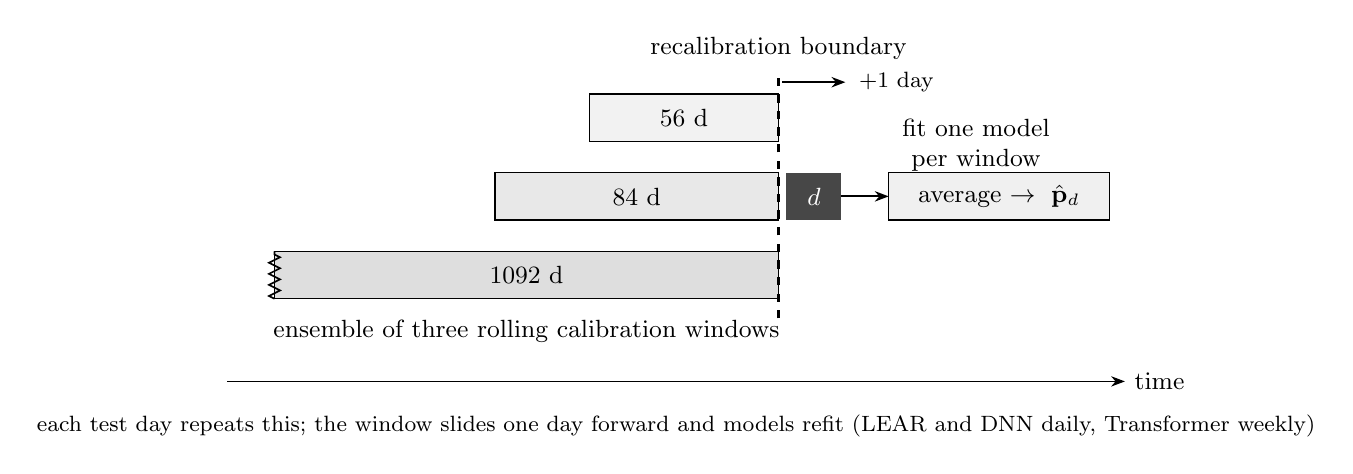
\begin{tikzpicture}[
  >={Stealth[length=5pt]},
  lbl/.style={font=\small},
  arr/.style={->, thick},
]
\def\bx{8}   % recalibration boundary (end of training data, start of target day)

% --- calibration-window bars (right edge at the boundary) ---
\fill[gray!10] (5.6,2.1) rectangle (\bx,2.7); \draw (5.6,2.1) rectangle (\bx,2.7);
\node[lbl] at (6.8,2.4) {56 d};
\fill[gray!18] (4.4,1.1) rectangle (\bx,1.7); \draw (4.4,1.1) rectangle (\bx,1.7);
\node[lbl] at (6.2,1.4) {84 d};
\fill[gray!26] (1.6,0.1) rectangle (\bx,0.7); \draw (1.6,0.1) rectangle (\bx,0.7);
\node[lbl] at (4.8,0.4) {1092 d};
% zigzag break: the long window really begins far to the left
\draw[decorate, decoration={zigzag, segment length=4pt, amplitude=2pt}, line width=0.6pt]
     (1.6,0.1) -- (1.6,0.7);

\node[lbl, align=center, anchor=north] at (4.8,-0.05)
   {ensemble of three rolling calibration windows};

% --- recalibration boundary ---
\draw[dashed, thick] (\bx,-0.15) -- (\bx,3.0);
\node[lbl, align=center, anchor=south] at (\bx,3.02) {recalibration boundary};
% slide indicator
\draw[arr] (\bx+0.05,2.85) -- (\bx+0.85,2.85);
\node[lbl, anchor=west, font=\footnotesize] at (\bx+0.9,2.85) {$+1$ day};

% --- target day cell ---
\fill[black!72] (8.1,1.1) rectangle (8.8,1.7);
\node[lbl, text=white] at (8.45,1.4) {$d$};

% --- fit + average ---
\node[lbl, align=center, anchor=west] at (9.45,2.05) {fit one model\\per window};
\fill[gray!12] (9.4,1.1) rectangle (12.2,1.7); \draw (9.4,1.1) rectangle (12.2,1.7);
\node[lbl, align=center] at (10.8,1.4) {average $\to\ \hat{\mathbf p}_{d}$};
\draw[arr] (8.8,1.4) -- (9.4,1.4);

% --- time axis ---
\draw[->] (1.0,-0.95) -- (12.4,-0.95) node[right,lbl]{time};

% --- walk-forward note ---
\node[lbl, align=center, anchor=north, font=\footnotesize] at (6.7,-1.25)
  {each test day repeats this; the window slides one day forward and models refit
   (LEAR and DNN daily, Transformer weekly)};

\end{tikzpicture}
\end{document}
